\documentclass{standalone}
\usepackage{tikz}
\usepackage{amsmath}
\begin{document}

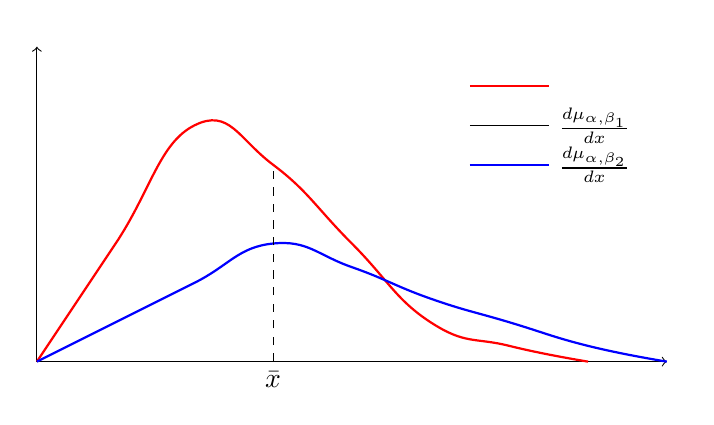
\begin{tikzpicture}
    % Axes
    \draw[->] (0,0) -- (8,0) node[right] {};
    \draw[->] (0,0) -- (0,4) node[above] {};

    % Red curve
    \draw[red, thick] plot[smooth, tension=0.8] coordinates {(0,0) (1,1.5) (2,3) (3,2.5) (4,1.5) (5,0.5) (6,0.2) (7,0)};
    
    % Blue curve
    \draw[blue, thick] plot[smooth, tension=0.8] coordinates {(0,0) (1,0.5) (2,1) (3,1.5) (4,1.2) (5,0.8) (6,0.5) (7,0.2) (8,0)};
    
    % Dashed line
    \draw[dashed] (3,0) -- (3,2.5);
    \node[below] at (3,0) {$\bar{x}$};
    
    % Legend
    \draw (5.5,3) -- (6.5,3) node[right] {\small$\frac{d\mu_{\alpha,\beta_1}}{dx}$};
    \draw[red, thick] (5.5,3.5) -- (6.5,3.5);
    \draw (5.5,2.5) -- (6.5,2.5) node[right] {\small$\frac{d\mu_{\alpha,\beta_2}}{dx}$};
    \draw[blue, thick] (5.5,2.5) -- (6.5,2.5);

\end{tikzpicture}

\end{document}